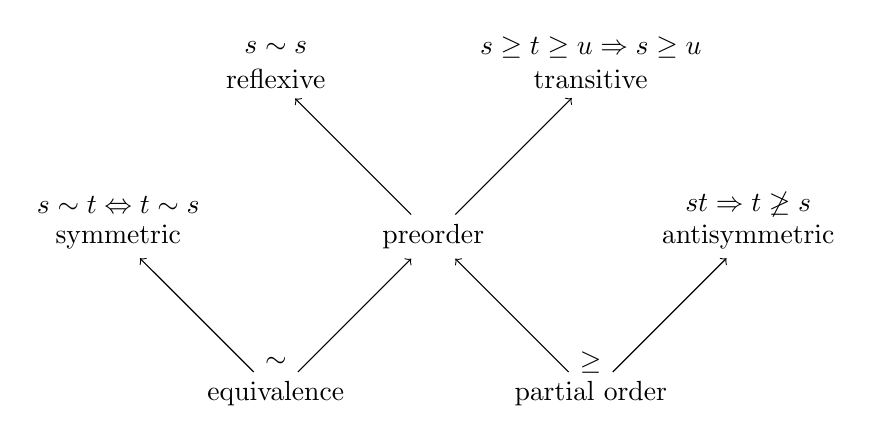
\begin{tikzpicture}

        \node (defSYMMETRIC) at (-4,0.4) { $s\sim t\Leftrightarrow t\sim s$ };
        \node (SYMMETRIC) at (-4,0) { symmetric };

            \node (defREFLEXIVE) at (-2,2.4) { $s\sim s$ };
            \node (REFLEXIVE) at (-2,2) { reflexive };

                \node (defTRANSITIVE) at (2,2.4) { $s\geq t\geq u\Rightarrow s\geq u$ };
                \node (TRANSITIVE) at (2,2) { transitive };

                    \node (defANTISYMMETRIC) at (4,0.4) { $s\gneq t \Rightarrow t\not\geq s$ };
                    \node (ANTISYMMETRIC) at (4,0) { antisymmetric };

        \node (PREORDER) at (0,0) { preorder };

    \node (SIM) at (-2,-1.6) { $\sim$ };
    \node (EQUIVALENCE) at (-2,-2) { equivalence };

    \node (GEQ) at (2,-1.6) { $\geq$ };
    \node (PARTIAL) at (2,-2) { partial order };

    % \node (PROPER) at (5,-1.5) { proper order };

    \draw[->] (PREORDER) -- (REFLEXIVE);
    \draw[->] (PREORDER) -- (TRANSITIVE);

    \draw[->] (EQUIVALENCE) -- (SYMMETRIC);
    \draw[->] (EQUIVALENCE) -- (PREORDER);
    \draw[->] (PARTIAL) -- (PREORDER);
    \draw[->] (PARTIAL) -- (ANTISYMMETRIC);

    % \draw[->] (PROPER) -- (TRANSITIVE);
\end{tikzpicture}